\documentclass{assignment}
\UsingEnglish
\ProjectInfos*{Intro to Communication System}{EE140}{Fall, 2020}{Assignment 9}{Due time : 10:15, Dec 4, 2020 (Friday)}{陈稼霖}{45875852}
\begin{document}
\begin{prob}[3.1]
    Let $U$ be an analog rv uniformly distributed between $-1$ and $1$.
    \begin{itemize}
        \item[(a)] Find the $3$-bit ($M=8$) quantizer that minimizes the MSE.
        \item[(b)] Argue that your quantizer satisfies the necessary condition for optimality.
        \item[(c)] Show that the quantizer is unique in the sense that no other $3$-bit quantizer satisfies the necessary condition for optimality.
    \end{itemize}
\end{prob}
\begin{sol}
    \begin{itemize}
        \item[(a)] 
        \item[(b)] 
        \item[(c)] 
    \end{itemize}
\end{sol}

\begin{prob}[3.3]
    Consider a binary scalar quantizer that partitions the set of reals $\mathbb{R}$ into two subsets $(-\infty,b)$ and $(b,\infty)$ and then presents $(-\infty,b]$ by $a_1\in\mathbb{R}$ and $(b,\infty)$ by $a_2\in\mathbb{R}$. This quantizer is used on each letter $U_n$ of a sequence $\cdots,U_1,U_0,U_1,\cdots$ of iid random variables, each having the probability density $f(u)$. Assume throughout this exercise that $f(u)$ is symmetric, i.e. that $f(u)=f(-u)$ for all $u\geq 0$.
    \begin{itemize}
        \item[(a)] Given the representation levels $a_1$ and $a_2>a_1$, how should $b$ be chosen to minimize the mean-squared distortion in the quantization? Assume that $f(u)>0$ for $a_1\leq u\leq a_2$ and explain why this assumption is relevant.
        \item[(b)] Given $b\geq 0$, find the values of $a_1$ and $a_2$ that minimize the mean-squared distortion. Given both answer in terms of the two functions $Q(x)=\int_x^{\infty}f(u)\,\mathrm{d}u$ and $y(x)=\int_x^{\infty}uf(u)\,\mathrm{d}u$.
        \item[(c)] Show that for $b=0$, the minimizing values of $a_1$ and $a_2$ satisfy $a_1=-a_2$.
        \item[(d)] Show that the choice of $b$, $a_1$, and $a_2$ in part (c) satisfies the Lloyd-Max conditions for minimum mean-squared distortion.
        \item[(e)] Consider the particular symmetric density
        \begin{figure}[H]
            \centering
            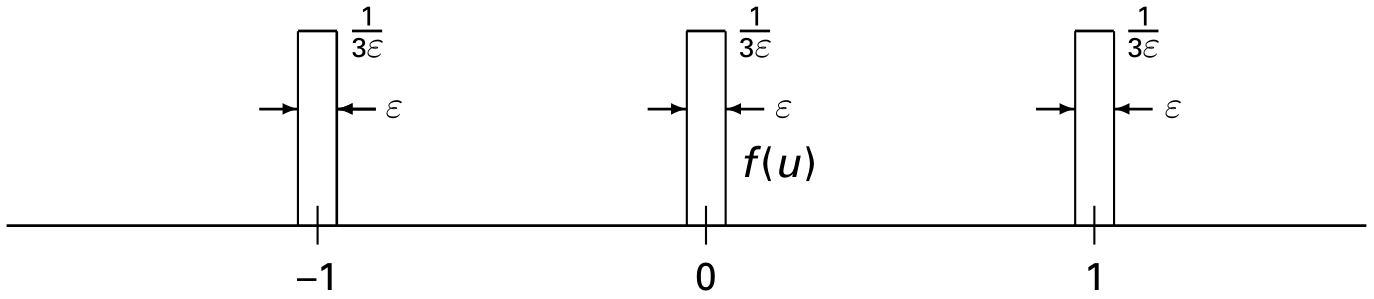
\includegraphics[width=.5\columnwidth]{A-9-P-1.png}
            \caption{}
            \label{A-9-P-1}
        \end{figure}
        Find all sets of triples $\{b,a_1,a_2\}$ that satisfy the Lloyd-Max conditions and evaluate the MSE for each. You are welcome in your calculation to replace each region of nonzero probability density above with an impulse, i.e. $f(u)=(1/3)[\delta(-1)+\delta(0)+\delta(1)]$, but you should use Figure \ref{A-9-P-1} to resolve the ambiguity about regions that occurs when $b$ is $-1,0$ or $+1$.
        \item[(f)] Given the MSE for each of your solutions above (in the limit of $\varepsilon\rightarrow 0$). Which of your solutions minimizes the MSE?
    \end{itemize}
\end{prob}
\begin{sol}
    \begin{itemize}
        \item[(a)] 
        \item[(b)] 
        \item[(c)] 
        \item[(d)] 
        \item[(e)] 
        \item[(f)] 
    \end{itemize}
\end{sol}

\begin{prob}[3.4]
    Section 3.4 partly analyzed a minimum-MSE quantizer for a pdf in which $f_U(u)=f_1$ over an interval of size $L_1$, $f_U(u)=f_2$ over an interval of size $L_2$, and $f_U(u)=0$ elsewhere. Let $M$ be the total number of representation points to be used, with $M_1$ in the first interval and $M_2=M-M_1$ in the second. Assume (from symmetry) that the quantization intervals are of equal size $\Delta_1=L_1/M_1$ in interval $1$ and of equal size $\Delta_2=L_2/M_2$ in interval $2$. Assume that $M$ is very large, so that we can approximately minimize the MSE over $M_1$, $M_2$ without an integer constraint on $M_1$, $M_2$ (that is, assume that $M_1$, $M_2$ can be arbitrary real numbers).
    \begin{itemize}
        \item[(a)] Show that the MSE in minimized if $\Delta_1f_1^{1/3}=\Delta_2f_2^{1/3}$, i.e. the quantization interval sizes are inversely proportional to the cube root of the density. [Hint. Use a Lagrange multiplier to perform the minimization. That is, to minimize a function MSE$(\Delta_1,\Delta_2)$ subject to a constraint $M=f(\Delta_1,\Delta_2)$, first minimize MSE$(\Delta_1,\Delta_2)+\lambda f(\Delta_1,\Delta_2)$ without the constraint, and, second, choose $\lambda$ so that the solution meets the constraint.]
        \item[(b)] Show that the minimum MSE under the above assumption is given by
        \[
            \text{MSE}=\frac{(L_1f_1^{1/3}+L_2f_2^{1/3})^3}{12M^2}.
        \]
        \item[(c)] Assume that the Lloyd-Max algorithm is started with $0<M_1<M$ representation points in the first interval and $M_2=M-M_1$ points in the second interval. Explain where the Lloyd-Max algorithm converges for this starting point. Assume from here on that the distance between the two intervals is very large.
        \item[(d)] Redo part (c) under the assumption that the Lloyd-Max algorithm is started with $0<M_1<M-2$ representation points in the first interval, one point between the two intervals, and the remaining points in the second interval.
        \item[(e)] Express the exact minimum MSE as a minimum over $M-1$ possibilities, with one term for each choice of $0<M_1<M$. (Assume there are no representation points between the two intervals.)
        \item[(f)] Now consider an arbitrary choice of $\Delta_1$ and $\Delta_2$ (with no constraint on $M$). Show that the entropy of the set of quantization points is given by
        \[
            H(V)=-f_1L_1\log(f_1\Delta_1)-f_2L_2\log(f_2\Delta_2).
        \]
        \item[(g)] Show that if the MSE is minimized subject to a constraint on the entropy (ignoring the integer constraint on quantization level), then $\Delta_1=\Delta_2$.
    \end{itemize}
\end{prob}
\begin{sol}
    \begin{itemize}
        \item[(a)] 
        \item[(b)] 
        \item[(c)] 
        \item[(d)] 
        \item[(e)] 
        \item[(f)] 
        \item[(g)] 
    \end{itemize}
\end{sol}

\begin{prob}[3.5]
    \begin{itemize}
        \item[(a)] Assume that a continuous-valued rv $Z$ has probability density that is $0$ except over the interval $[-A,+A]$. Show that the differential entropy $h(Z)$ is upperbounded $1+\log_2A$.
        \item[(b)] Show that $h(Z)=1+\log_2A$ if and only if $Z$ is uniformly distributed between $-A$ and $+A$.
    \end{itemize}
\end{prob}
\begin{sol}
    \begin{itemize}
        \item[(a)] 
        \item[(b)] 
    \end{itemize}
\end{sol}
\end{document}